\chapter{Clustering e Topic Modelling, LLM e Prompting}

\section{Clustering Testuale con Embeddings}

\paragraph{La pipeline per il Clustering Testuale si articola in tre fasi:}

\begin{enumerate}
  \item Conversione dei documenti in vettori (\textit{embeddings}): su \fancyglitter{Hugging Face} è disponibile un modello pre-addestrato chiamato \textit{General Text Embeddings} (GTE). 
  \item Riduzione della dimensionalità degli embeddings: dato che gli embeddings hanno dimensioni elevate è necessario ridurli, per esempio con \fancyglitter{UMAP}. 
  \item Clustering dei vettori in gruppi significativi: per raggruppare documenti simili, si può usare \fancyglitter{HDBSCAN}.
\end{enumerate}

\nt {Successivamente c'è la fase di visualizzazione dei risultati (fig: \ref{fig:vis}), come visto in precedenza.}

\begin{figure}[h]
    \centering
    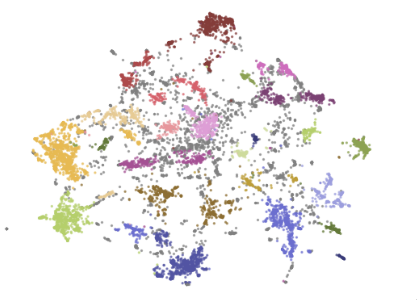
\includegraphics[scale=0.75]{04/visual.png}
    \caption{Visualizzazione dei dati.}
    \label{fig:vis}
\end{figure}

\subsection{BERTopic}

\dfn{BERTopic}{
  BERTopic è un framework moderno per il topic modelling. Si basa su:
  \begin{itemize}
    \item Una pipeline di clustering su embeddings testuali. 
    \item L'estrazione di parole salienti per ogni cluster attraverso \textit{class-based TF-IDF}.
  \end{itemize}
}

\paragraph{È possibile accedere alle informazioni dei topic estratti con i comandi:}

\begin{itemize}
  \item \texttt{topic\_model.get\_topic\_info()}. 
  \item \texttt{topic\_model.get\_topic()}.
\end{itemize}

\paragraph{Sono supportate diverse funzioni di interrogazione e visualizzazione:}

\begin{itemize}
  \item Ricerca di topic associati a una query. 
  \item Diagrammi interattivi: 
    \begin{itemize}
      \item \texttt{visualize\_documents()}. 
      \item \texttt{visualize\_barchart()}. 
      \item \texttt{visualize\_hierarchy()}. 
      \item \texttt{visualize\_heatmap()}.
    \end{itemize}
\end{itemize}

\section{LLM e Prompting}

Gli LLMs sono modelli di intelligenza artificiale utilizzati per generare testi. Ne esistono di vari tipi, una prima distinzione può essere in:

\begin{itemize}
  \item \fancyglitter{Basici:} in grado di generare testo tramite predizioni statistiche ma non in grado di rispondere a domande specifiche. 
  \item \fancyglitter{Instructed:} addestrati con domande e risposte. Possono essere guidati in direzioni specifiche.
\end{itemize}

\subsection{Prompting}

\dfn{Prompting}{
  Il prompting è il processo che consiste nel fornire al modello di intelligenza artificiale un input specifico per guidarlo nella generazione di un output desiderato.
}

\paragraph{Linee guida del prompting:}

\begin{itemize}
  \item Istruzioni chiare e specifiche: è importante fornire al modello di IA delle istruzioni chiare per comprendere esattamente ciò che gli si sta chiedendo. 
  \item Uso dei segni di punteggiatura: per specificare meglio le richieste è necessario usare una corretta punteggiatura. 
  \item Richiesta di formato di output: si può specificare il formato con cui si vuole restituito l'output.
  \item Iterative Prompting Development: è possibile raffinare il processo di prompting attraverso un approccio iterativo.
\end{itemize}

\paragraph{Strategie di prompting:}

\begin{itemize}
  \item Prompting basato su sequenze di istruzioni: si può usare il prompting per fornire al modello una serie di istruzioni.
  \item Prompting iterativo: si può chiedere al modello di eseguire $n$ ministep per arrivare a una conclusione.
  \item Prompting basato su dialoghi: se l'input è il dialogo tra più persone si può usare il prompting per continuarlo.
  \item Forza il modello a ragionare in "modo piano": si forza il modello a effettuare una serie di ragionamenti prima di fornire la risposta.
  \item \textit{Chain of Thought} (CoT): richiesta di feedback, per fare in modo che il modello segnali eventuali errori o imprecisioni.
\end{itemize}

\subsection{Summarization e Inferenza}

Come accennato in precedenza gli LLMs possono essere usati per riassumere testi tenendo intatto il significato originale. Questo processo avviene attraverso la generazione di un testo di output che contiene le informazioni più rilevanti di un testo di input. Questa sintesi può essere personalizzata specificando il numero di token, frasi o caeratteri, etc. Inoltre è possibile specializzare l'output, concentrandosi solo su particolari caeratteristiche. 

Un altro utilizzo consiste enll'utilizzare gli LLMs per fare inferenza e \textit{sentiment analysis} (capire se un certo testo è positivo o meno su un determinato argomento).  Tradizionalmente la sentiment analysis veniva fatta annotando manualmente testi e creando modelli di classificazione. Attualmente può essere gestito tutto a livello di prompting.

\clm{}{}{
  \begin{itemize}
    \item È possibile richiedere informazioni in modo flessibile e personalizzabile.
    \item Si possono usare LLMs per trovare gli argomenti principali di un testo.
  \end{itemize}
}

\subsection{Trasformazione ed Espansione}

Gli LLMs possono anche essere usati per trasformare dei testi: cambiare formato, tradurli, cambiare stile, etc. 

\paragraph{Task di trasformazione:}

\begin{itemize}
  \item Traduzione: uno dei principali, si può anche rilevare automaticamente la lingua. 
  \item Trasformare lo stile: da formale a informale e viceversa. 
  \item Trasformare da JSON a HTML, etc, correzione di errori ortografici, etc.
\end{itemize}

Una delle applicazioni più potenti degli LLMs è l'espansione: consentire agli utenti di allungare del contenuto in input. L'utente fornisce al modello un testo e il modello usa la sua comprensione del linguaggio e del contesto per generare altro testo. Un esempio: un utente fornisce un insieme schematico di punti e chiede al modello di generare un email partendo da essi. Quando si vuole genere testo si deve anche tenere conto della \fancyglitter{temperatura}. 

\dfn{Temperatura}{
  La temperatura è un parametro che controlla la variabilità dell'output: con temperatura bassa il modello genera risposte prevedibili, con temperatura alta diventa "creativo".
}

\qs{}{Perché la temperatura è importante?}

\begin{itemize}
  \item Per documenti tecnici è preferibile un output preciso, quindi con temperatura bassa. 
  \item Per la scrittura creativa e il copywriting viene preferita una temperatura alta.
\end{itemize}

Un'ennesima applicazione degli LLMs è quella di usarli come sistemi di ricerca. Esistono vari approcci:

\begin{itemize}
  \item Utilizzare prompt basati su NLP che imitano gli esseri umani. 
  \item Utilizzare prompt specifici e dettagliati, fornendo ulteriore contesto e vincoli. 
\end{itemize}

\nt{Gli LLMs hanno limiti per questi compiti: possono produrre errori o risultati non pertinenti. Un altro problema consiste nel fatto che si può fare retrieval di informazioni non aggiornate.}

\subsection{Aspetti Pratici del Prompting}

\paragraph{Il prompting riguarda diverse componenti:}

\begin{itemize}
  \item Istruzioni: una specifica attività che il modello deve seguire. Si devono testare vari tipi di istruzioni per trovare quelle più adatte al proprio scopo.
  \item Contesto: include informazioni esterne. 
  \item Input di dati: si riferisce all'input o alla domanda. 
  \item Indicatore di output: indica il tipo e il formato di output. 
\end{itemize}

\nt{Un altro suggerimento è quello di evitare le negazioni.}

\paragraph{Specifiche ulteriori:}

\begin{itemize}
  \item \fancyglitter{Zero-shot:} non si fornisce alcun suggerimento riguardo ciò che ci si aspetta. 
  \item \fancyglitter{Few-shot:} si specifica cosa si intende con una determinata etichetta e cosa ci si aspetta in output. 
  \item \fancyglitter{Chain of Thought:} si richiede al modello di esplicitare i passaggi svolti per aumentare le performance.
\end{itemize}

\section{RAG e Chunking}

Uno dei limiti degli LLMs è che non sempre dispongono di informazioni aggiornate o specifiche. Per cui si introduce un nuovo paradigma \fancyglitter{Retrieval-Augmented Generation} (RAG) che combina la generazione degli LLMs con il recupero da fonti precise o database.

\qs{Che cos'è il RAG?}

\paragraph{Il RAG si basa su:}

\begin{itemize}
  \item \fancyglitter{Retrieval:} il sistema usa un motore di ricerca interno per individuare i documenti. 
  \item \fancyglitter{Generation:} i documenti vengono forniti al LLM come contesto per generare una risposta.
\end{itemize}

\subsection{Il Chunking}

\dfn{Chunking}{
  Il chunking consiste nella suddivisione dei documenti testuali in blocchi (chunk) di dimensioni gestibili, da indicizzare e recuperare successivamente. 
}

\paragraph{Aspetti chiave del chunking:}

\begin{itemize}
  \item \fancyglitter{Dimensione:} un chunk troppo lungo può superare il limite di contesto del modello, ma uno troppo breve è poco informativo. Solitamente è tra 200 e 500 token. 
  \item \fancyglitter{Sovrapposizione (overlap):} si prevede sovrapposizione tra chunk adiacenti per evitare di perdere informazioni nei punti di separazione. 
    \item \fancyglitter{Segmentazione intelligente:} i chunk non devono interrompere a metà frasi e concetti.
\end{itemize}

\paragraph{Metodi di chunking:}

\begin{itemize}
  \item A livello di token/carattere: semplice, ma inefficace a livello semantico. 
  \item A livello di frase: mantiene l'integrità delle frasi, migliora la coerenza. 
  \item Semantico: sfrutta tecniche di \textit{sliding windows} e calcolo della divergenza per individuare confini nei contenuti. 
\end{itemize}

\nt{Dopo aver generato i chunk è necessario convertirli in vettori tramite modelli di embedding e salvarli in un indice vettoriale. Quando l'utente pone una domanda essa viene trasformata in embedding e confrontata (in genere con la cosine similarity).}

\subsection{Vantaggi e Limitazioni del RAG}

\paragraph{Prompting nel RAG:}

\begin{itemize}
  \item Si delimita chiaramente il contesto fornito. 
  \item Si specifica che la risposta deve essere limitata al contesto dato. 
  \item Si indica il formato dell'output.
\end{itemize}

\paragraph{Vantaggi e limiti:}

\begin{itemize}
  \item [\textcolor{green}{\ding{51}}] Aggiornabilità: si può facilmente aggiornare fornendo nuovi documenti. 
 \item [\textcolor{green}{\ding{51}}] Controllo sulle fonti: l'utente o l'organizzazione ha un controllo diretto sulle fonti utilizzate, questo permette un comportamento più prevedibile e personalizzabile.
    \item [\textcolor{green}{\ding{51}}] Tracciabilità delle risposte: si possono fornire riferimenti diretti alle fonti utilizzate. 
       \item [\textcolor{red}{\ding{55}}] Rischio di falsa sicurezza: il modello può comunque generare informazioni sbagliate (allucinazioni). 
          \item [\textcolor{red}{\ding{55}}] Limitazioni del contesto: anche se vengono recuperati molti chunk pertinenti solo una parte andrà a costituire la risposta. 

             \item [\textcolor{red}{\ding{55}}] Dipendenza dalla quantità del retrieval: l'efficacia del sistema dipende da quanto può recuperare informazioni. 
\end{itemize}

